\chapter{Dynamic Transport Services \who{Maciejewski}}
\label{ch:dts}
% ##################################################################################################################

\hfill \textbf{Author:} Michal Maciejewski

\begin{center} 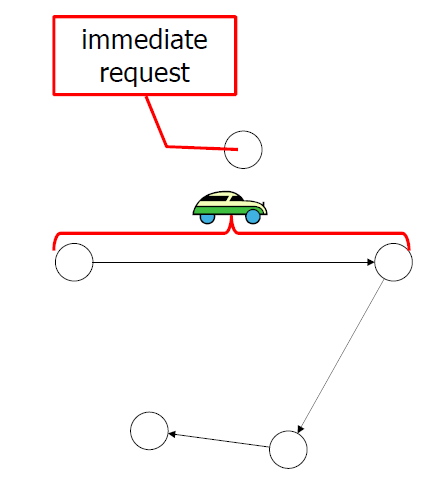
\includegraphics[width=0.4\textwidth, angle=0]{extending/figures/DTS/dts.png} \mm{change this picture} \end{center}

\section{Introduction}

DTS - there is a gap.

General info on MATSim's DVRP extension. Assumptions, applications...

Agents are dynamic.

\section{DynAgent}

The \lstinline$DynAgent$ class, along with the \lstinline$org.matsim.contrib.dynagent$ package, provides the foundation for MATSim's DVRP extension by adding dynamism to the behavior of agents. The main idea behind \lstinline$DynAgent$ is that instead of using a pre-computed (and occasionally re-computed; see \ref{sec:impl-plan-based}) plan, an agent can actively decide what to do at each simulation step. It is up to the agent, whether decisions are made on the fly or (re-)planned in advance. In some applications, a \lstinline$DynAgent$ may represent a fully autonomous agent that acts according to his/her desires, beliefs and intentions, whereas in other cases, it may a non-autonomous agent following orders that are systematically coming from the outside (e.g. a driver receiving tasks from a centralized vehicle dispatching system).

\subsection{Main interfaces and classes}

The \lstinline$DynAgent$ class is a dynamic implementation of \lstinline$MobsimDriverPassengerAgent$. Instead of executing pre-planned \lstinline$Activity$s and \lstinline$Leg$s, a \lstinline$DynAgent$ performs \lstinline$DynActivity$s and \lstinline$DynLeg$s. The following assumptions underlie the agent's behavior:
%
\begin{itemize}
	\item the \lstinline$DynAgent$ is the physical representation of the agent, responsible for the interaction with the real world (i.e., traffic simulation)

	\item the agent's high-level behavior is controlled by a \lstinline$DynAgentLogic$ that can be seen as the agent's brain; the \lstinline$DynAgentLogic$ is responsible for deciding on the agent's next action (leg or activity) once the current one has ended
	
	\item dynamic legs and activities fully define the agent's low-level behavior, down to the level of a single step in simulation.
\end{itemize}
%
At the higher level, the dynamism of the \lstinline$DynAgent$ results from the fact that dynamic activities and legs are usually created on the fly by the agent's \lstinline$DynAgentLogic$, thus the agent does not have to plan future actions in advance. In the case when the agent has a more or less detailed plan of legs and activities, the agent does not have to adhere to it, and may modify his/her plan at any time (e.g., change the mode or destination of a future leg, or include or omit a future activity).

The low-level dynamism is provided by the mechanism of executing dynamic activities and legs. As for the currently executed activity, the agent can shorten or lengthen its duration at any time. Additionally, at each time step, the agent may decide upon what to do right now (e.g., communicate with other agents, re-plan the next activity or leg, and so on). In the case of driving a car (\lstinline$DriverDynLeg$), the agent can change the route, destination or even decide upon picking up or dropping off somebody on the way. When using the public transport (\lstinline$PTPassengerDynLeg$), the agent chooses which bus to get on and which stop to exit at.

Incidentally, the behavior of MATSim's default plan-based agent, \lstinline$PersonDriverAgentImpl$, can be simulated by \lstinline$DynAgent$ combined with the \lstinline$PlanToDynAgentLogicAdapter$ logic. This adapter class creates series of dynamic activities and legs that mimics a given \lstinline$Plan$ of static \lstinline$Activity$s and \lstinline$Leg$s.

\subsection{Configuring and running a dynamic simulation}
\label{sec:config-dyn-sim}

\lstinline$DynAgent$ has been written for and validated aginst \lstinline$QSim$. Simulation of dynamic legs does not require any additional code. However, to take advantage of dynamic activities,  \lstinline$DynActivityEngine$ should be used instead of \lstinline$ActivityEngine$. \lstinline$DynActivityEngine$'s \lstinline$doSimStep(double time)$ method ensures that dynamic activities are actively executed by agents and their end times can be changed.

The easiest way to run a single iteration of \lstinline$QSim$ is as follows:
%
\begin{enumerate}

	\item Call \lstinline$DynAgentLauncherUtils$' \lstinline$initQSim(Scenario scenario)$ method to create and initialize a \lstinline$QSim$; this includes creating a series of objects, such as an \lstinline$EventMananger$, \lstinline$DynActivityEngine$, or \lstinline$TeleportationEngine$

	\item Add \lstinline$AgentSource$s of \lstinline$DynAgent$s and other agents to the \lstinline$QSim$
	
	\item Run simulation by calling \lstinline$QSim$'s \lstinline$run()$ method
	
	\item Finalize processing events by calling \lstinline$EventManager$'s \lstinline$finishProcessing()$ method
	
\end{enumerate}
%
Depending on the needs, the above procedure can be extended with additional steps, such as adding non-default engines or departure handlers to the \lstinline$QSim$.

\subsection{Example}

The \lstinline$org.matsim.contrib.dynagent.examples.random$ package contains a basic illustration of how to create and run a scenario with \lstinline$DynAgent$s. To highlight the contrast to the plan-based agents, in this example, 100 dynamic agents travel randomly (\lstinline$RandomDynLeg$) and perform activities of random duration (\lstinline$RandomDynActivity$).

The high-level random behavior is controlled by \lstinline$RandomDynAgentLogic$ that operates according to the following rules:
%
\begin{enumerate}

	\item Each agent starts with a \lstinline$RandomDynActivity$; see the \lstinline$computeInitialActivity(DynAgent agent)$ method
	
	\item Whenever the currently performed activity or leg ends, a random choice on what to do next is made between the following options: (a) stop being simulated by starting a deterministic \lstinline$StaticDynActivity$ with infinite end time, (b) start a \lstinline$RandomDynActivity$, or (c) start a \lstinline$RandomDynLeg$; see the \lstinline$computeNextAction(DynAction oldAction, double now)$ method

\end{enumerate}

The stochasticity at the lower level results from random decisions being made at each consecutive decision point. In the case of \lstinline$RandomDynLeg$, each time an agent enters a new link, he or she decides whether to stop at this link or to continue driving; in the latter case, the subsequent link is chosen randomly; see the \lstinline$RandomDynLeg(Id<Link> fromLinkId, Network network)$ constructor and the \lstinline$movedOverNode(Id<Link> newLinkId)$ method. As for \lstinline$RandomDynActivity$, at each time step, the \lstinline$doSimStep(double now)$ method is called and a random decision is made on the activity end time.

Following the rules specified in Sec.~\ref{sec:config-dyn-sim}, setting up and running this example scenario is straightforward. \lstinline$RandomDynAgentLauncher$ reads a network, initializes a \lstinline$QSim$, then adds a \lstinline$RandomDynAgnetSource$ to the \lstinline$QSim$, and finally, launches visualization and starts simulation. The \lstinline$RandomDynAgentSource$ is responsible for instantiating 100 \lstinline$DynAgent$s that are randomly distributed over the network. The simulation ends when the last active agent becomes inactive.

\section{VRP}










% ##################################################################################################################
Joschka Bischoff as author?
Taxis Berlin: electric vehicles -> pres Wiepersdorf

Mielec and Berlin Scenarios

http://www.matsim.org/node/379

\kwaah{does MATSim 2030 help here?}

% ##################################################################################################################